\section{バックアップ}\label{s1:バックアップ} %{
\begin{description}\setlength{\itemsep}{-1mm} %{
	%
	\item[級数展開] M\"obius変換を明示的に示す級数展開を導く。
	\eqref{eq:rho-int-1}の積分変数を次のように変換する。
	\begin{alignat*}{2}
		\rho(\beta|x) 
		&= \sigma(x)^{-\beta}\int_0^{\sigma(x)} d(s^\beta)\sigma^{-1}(s)
		&\quad&\text{// } s = \sigma(z),\;\sigma^{-1}(s) = \frac{s}{1 + s} \\
		&= \sigma(x)^{-\beta}\int_0^{\sigma(x)^\beta} dt\sigma^{-1}(t^{\frac{1}{\beta}})
		&\quad&\text{// } t = s^\beta
	\end{alignat*}
	$\sigma^{-1}(t^{1/\beta})$を$t^{1/\beta}=0$近傍でべき展開するが、$x$の値に
	よって場合分けする必要がある。
	\begin{description}\setlength{\itemsep}{-1mm} %{
		\item[$x\le 1/2$の時] この時は、$\sigma(x)\le 1$となり、被積分変数$t$が
		$|t|<1$となり、次のようにべき展開できる。
		\begin{equation*}
			\rho(\beta|x) = \sigma(x)^{-\beta}\int_0^{\sigma(x)^\beta} dt 
				t^{\frac{1}{\beta}}\sum_{n\in\sizen} \plra{- t^{\frac{1}{\beta}}}
			= \beta \sum_{n\in\sizen} (-)^n\frac{\sigma(x)^{n + 1}}{\beta + n + 1}
		\end{equation*}
		%
		\item[$1/2< x$の時] この時は、$1<\sigma(x)$となり、被積分変数$t$が
		$|t|<1$ではなくなり、積分範囲を分割する必要がある。
		\begin{equation*}\begin{split}
			\rho(\beta|x) 
			= \sigma(x)^{-\beta}\plra{\int_0^1 + \int_1^{\sigma(x)^\beta}} dt 
			\sigma^{-1}\plra{t^{\frac{1}{\beta}}}
		\end{split}\end{equation*}
		一つ目の積分は$x\le1/2$の場合と同じだが、二つ目の積分はべき展開が異なる。
		\begin{equation*}\begin{split}
			\sigma(x)^{-\beta}\int_1^{\sigma(x)^\beta}dt
				\sigma^{-1}\plra{t^{\frac{1}{\beta}}}
			&= \sigma(x)^{-\beta}\int_1^{\sigma(x)^\beta}dt
				\sum_{n\in\sizen}\plra{- t^{- \frac{1}{\beta}}}^n \\
			&= - \beta\sum_{n\in\sizen}(-)^n
				\frac{\sigma(x)^{- \beta} - \sigma(x)^{- n}}{\beta - n}
		\end{split}\end{equation*}
		$\beta\in\sizen$の場合、和の中に不定な項が現れるが、それは次の極限を
		とるものとする。
		\begin{equation*}
			\lim_{\beta\to n}\frac{\sigma(x)^{- \beta} - \sigma(x)^{- n}}{\beta - n}
			= - \lim_{\beta\to n}\sigma(x)^{- \beta}\ln\sigma(x)
			= - \frac{\ln\sigma(x)}{\sigma(x)^n}
		\end{equation*}
	\end{description} %}
	以上をまとめると、次の級数展開が得られる。
	\begin{equation}\label{eq:rho-int-mobius}
		\rho(\beta|x) = \beta\sum_{n\in\sizen}(-)^n\begin{cases}
			\cfrac{\sigma(x)^{n + 1}}{\beta + n + 1}
			, &\text{ if } |x| < \frac{1}{2} \\
			\cfrac{1}{\beta + n + 1} 
			- \cfrac{\sigma(x)^{- \beta} - \sigma(x)^{- n}}{\beta - n}
			, &\text{ otherwise } \\
		\end{cases}
	\end{equation}
\end{description} %}

\subsection{分岐を持つ複素積分} % (fold)
\label{sub:分岐を持つ複素積分}
単位円上の積分$\oint_{|z|=1}dzz^{\frac{1}{2}}$を考える。
円座標を使って計算すると次のようになる。
\begin{alignat*}{2}
	\oint_{|z|=1}dzz^{\frac{1}{2}}
	&= i\int_0^{2\pi} d\theta \exp\plra{\frac{3i}{2}\theta}
	&\quad&\text{// } z = \exp\plra{i\theta} \\
	&= \frac{2}{3}\blra{\exp\plra{\frac{3i}{2}\theta}}_{\theta=0}^{2\pi}
	= - \frac{4}{3}
\end{alignat*}
積分路の組み合わせを使って計算してみよう。図\ref{fig:積分路その一}のように、
$C_1$を$|z|=1$の反時計回りの円周、$C_\epsilon$を$|z|=\epsilon<1$の時計回りの円周、
$L_+$を$\epsilon$から$1$への実軸上の直線、$L_-$を$1$から$\epsilon$への実軸上の直線とし、
それらを繋げた閉路を$\Gamma$とする。
\begin{equation*}
	\oint_\Gamma = \int_{C_1} + \int_{L_-} + \int_{C_\epsilon} + \int_{L_+}
\end{equation*}
$dzz^{\frac{1}{2}}$の分岐を正の実軸にとると、$\Gamma$の内部には$dzz^{\frac{1}{2}}$の極と
分岐が無いので、$\oint_\Gamma dzz^{\frac{1}{2}}=0$となり、
$\lim_{\epsilon\to0}\int_{C_\epsilon}dzz^{\frac{1}{2}}=0$だから、次の式が成り立つ。
\begin{equation}\begin{split}\label{eq:branch-1}
	\int_{C_1}dzz^{\frac{1}{2}} 
	&= - \lim_{\epsilon\to0}\plra{\int_{L_-} + \int_{L_+}}dzz^{\frac{1}{2}} \\
	&= - \int_1^0 dze^{\pi i}z^{\frac{1}{2}} - \int_0^1 dzz^{\frac{1}{2}}
	= \int_1^0 dzz^{\frac{1}{2}} - \int_0^1 dzz^{\frac{1}{2}} = - \frac{4}{3}
\end{split}\end{equation}

\begin{figure}[htbp] %{
	\begin{center}
		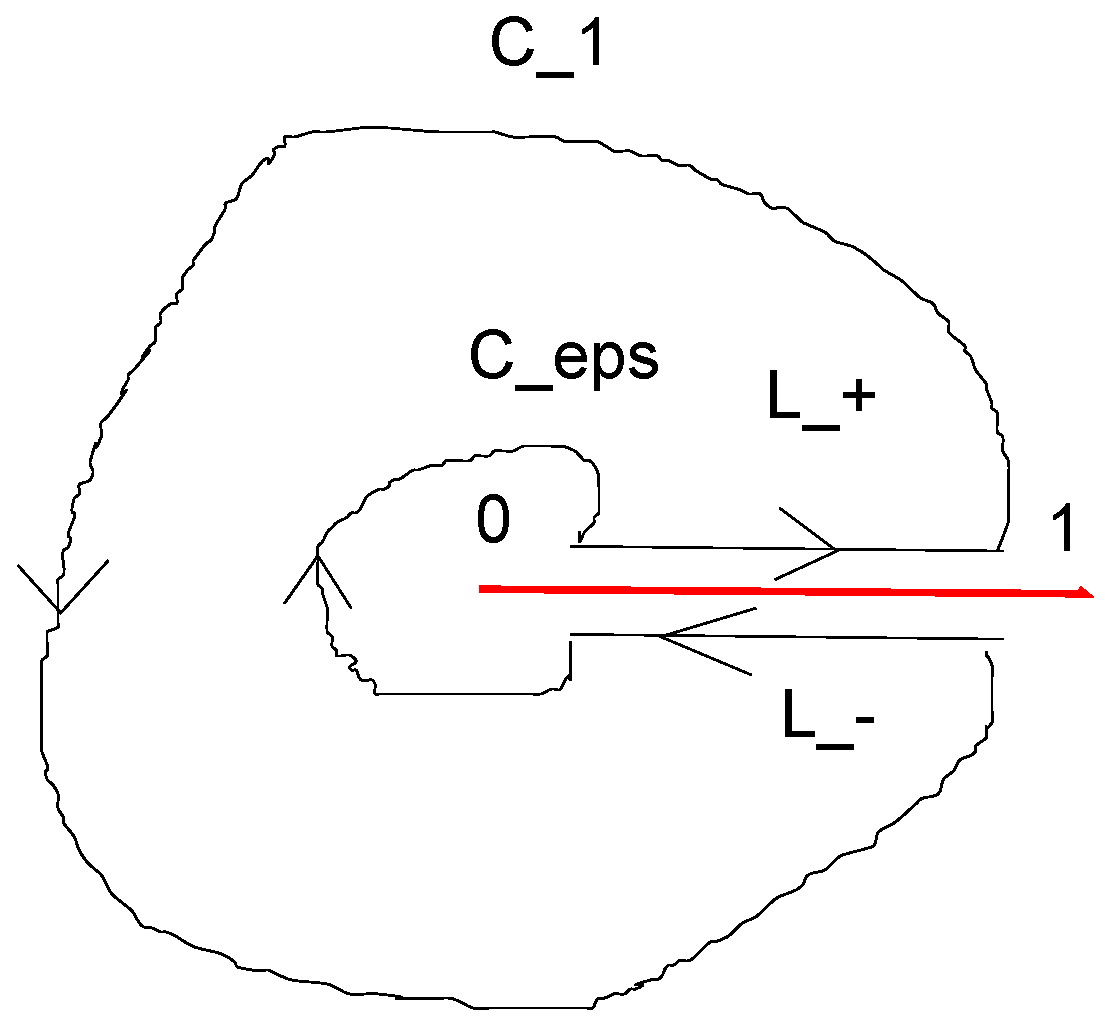
\includegraphics[width=0.3\textwidth]{fig/contour-1.eps}
	\end{center}
	\caption{積分路その一}\label{fig:積分路その一}
\end{figure} %}

$\int_1^z$の積分路によって$\ln z$の多意性$\ln z+2n\pi i$を表すことができる。
積分路が原点の周りを時計回りに一周する毎に、$2\pi i$ずつ$\ln z$に加算されて
いく。逆に、多意性を取り除くために、複素平面から原点を取り除き、原点から
無限遠点までハサミで切断した空間$K_0$を考え、$\int_1^z$の積分路を$K_0$内に
限定したものを$\ln z$と定義し、$z^a$を$e^{a\ln z}$によって定義する。
\eqref{eq:branch-1}の$L_-$による積分の被積分関数の因子$e^{\pi i}$は、
正の実軸を分岐切断として計算されたものになっている。

\cite{hb3.s6:online}\cite{www.e5:online}はリーマン面の簡潔な
イントロダクションだと思う。\cite{www.s3:online}は超幾何関数について古典的
な結果とそれを現代的な視点で捉え直したところまで網羅した概観を与えている。
% subsection 分岐を持つ複素積分 (end)
%s1:バックアップ}
